\section{Grupper (2)}
\subsection{Indledende gruppeteori (2.1)}
\subsubsection{Def. Komposition}
En komposition på en mængde G er en afbildning $\circ: G \times G \rightarrow G$.
Kompositionen $\circ(g, h)$ skrives ofte $g \circ h$ eller blot $gh$.

\subsubsection{Def. 2.1.1}
Et par, $(G, \circ)$, bestående af en mængde $G$ og en komposition $\circ: G
\times G \rightarrow G$ kaldes en \textit{gruppe} hvis den tilfredsstiller
følgende tre egenskaber:
\begin{enumerate}[(i)]
  \item Kompositionen skal være \textbf{associativ}:
  \begin{equation*}
  g_1 \circ (g_2 \circ g_3) = (g_1 \circ g_2) \circ g_3
  \end{equation*}
  for alle $g_1, g_2, g_3 \in G$
  
  \item Der skal eksistere et \textbf{neutralt} element $e \in G$, sådan at:
  \begin{equation*}
  e \circ g = g \quad \text{og}\quad g \circ e = g
  \end{equation*}
  for alle $g \in G$
  
  \item For alle $s \in G$ eksisterer der et \textbf{inverst} element $t \in G$, sådan
  at: 
  \begin{equation*}
  g \circ t = e \quad \text{og} \quad t \circ g = e
  \end{equation*}
\end{enumerate}
En gruppe $G$ kaldes abelsk hvis der for alle $x, y \in G$ gælder at $x \circ y
= y \circ x$. Antallet af elementer $|G|$ i $G$ kaldes ordnen af $G$.

\subsubsection{Def. 2.1.7}
Lad $g \in G$ være et element i en gruppe. Så er $g^{-1} \in G$ det entydige
inverse element til $g$.

\subsubsection{Finde inversen til et produkt}
Inversen til et produkt $ab \in G$ er $b^{-1}a^{-1}$ da:
\begin{equation*}
  (ab)(b^{-1}a^{-1}) = a(b(b^{-1}a^{-1})) = a(ea^{-1}) = aa^{-1} = e
\end{equation*}

\subsubsection{Kompositionstabel (2.1.2)}
Se. side 53.

\subsubsection{Gruppen $S_3$ (2.1.4)}
\label{S_3}
$S_3$ er gruppen bestående af de 6 bijektioner der findes for elementerne
$X = \{1,2,3\}$. Gruppens komposition er den normale komposition for
afbildninger, dvs. operationen $f(g(x))$, for bijektionerne $f, g \in G$.
\begin{enumerate}[(i)]
  \item Det neutrale element $e$ er identitetsafbildningen $X \rightarrow X$.
  \item Den inverse til en bijektion $f$ er den inverse afbildning $f^{-1}: X
  \rightarrow X$.
  \item Komposition af afbildninger er desuden assosiativ.
\end{enumerate}
Se s. 55 for eksempel og kompositionstabel.

\subsubsection{Multiplikation med $g \in G$ er bijektiv}
Antag $G$ er en gruppe og $g \in G$. Der eksisterer en afbildning
$\phi:G\rightarrow G$ givet ved $\phi(x) = gx$. Denne afbildning er bijektiv.

Vi kan vise $\phi$ er bijektiv, givet dens inverse, nemlig $\psi: G
\rightarrow G$. Denne afbildning er givet ved $\psi(x) = g^{-1}x$. Ved
komposition gælder nu:
\begin{enumerate}[(i)]
  \item $\psi(\phi(x)) = x$
  \item $\phi(\psi(x)) = x$
\end{enumerate}
Udregningerne er sparet væk (se s. 56). Afbildningen $\varepsilon : G
\rightarrow G$, givet ved $\varepsilon(x) = xg$ er også bijektiv og dette vises
på samme måde.

\textit{Enhver afbildning der har en invers er bijektiv.}

\subsubsection{Kvotientgruppen $\Z/n\Z$}
\label{kvotientgruppe}
$(\Z, +)$ er en gruppe. Vi definerer nu en kvotientgruppe til at være en gruppe
hvis elementer er restklasserne (\nameref{1.2.3}) for et givet $n \in \Z$:
\begin{equation*}
  \Z/n\Z = \myset{[0]_n,[1]_n,\ldots,[n-1]_n}
\end{equation*}
En restklasse er selv en mængde, derfor er en \textbf{kvotientgruppe en mængde af
mængder.}

En restklasse, $[a]_n$ kan udtrykkes på formen:
\begin{equation*}
  a + n\Z = \{a + nx | x \in \Z\}
\end{equation*}
hvor $a \in \Z$ er repræsentanten for klassen og $n \in Z$ er det tal vi regner
modulo.

\textit{Et eksempel: $[2]_5 = 2 + 5\Z = \{\ldots, -8, -3, 2, 7, \ldots\}$. Dvs.
mængden af alle tal der er kongruent med 2 modulo 5.}.
\\
\\
Fra \nameref{1.3.2} gælder der nu at hvis $n > 0$:
\begin{equation*}
  a + n\Z = b + n\Z \iff [a]_n = [b]_n
\end{equation*}
\textit{Der eksisterer kun $n-1$ entydige rester mht. $n$ (\nameref{1.2.1}).
Derfor er $[12]_5 = [2]_5$, da disse har fuldstændig samme rest mht. $n$. Vi bruger
derfor som regel kun repræsentanter fra $0,\ldots,n-1$ da de andre er
inkluderede heri.}

Nogle eksempler på specielle kvotientgrupper:
\begin{align*}
  &\Z/0\Z \Rightarrow \{x\} = x + 0\Z = x  \Rightarrow (\Z, +)\\
  &\Z/1\Z \Rightarrow \{[0]_1\} = 0 + 1\Z = (\Z, +)
\end{align*}

\subsubsection{Prop. 2.1.2}
\label{2.1.2}
Lad $a, b, n \in \Z$. Så gælder:
\begin{enumerate}[(i)]
  \item $a + n\Z = b + n\Z\\
  \iff a \mycong{b}{n}$

  \item $(a + n\Z) \cap (b + n\Z) = \emptyset\\
  \iff a \not \mycong{b}{n}$ 
\end{enumerate}
\textit{(i): Hvis $[a]_n = [b]_n$ så er $a$ og $b$ kongruente modulo $n$ og vice
versa. (ii): Hvis $[a]_n$ og $[b]_n$ ingen elementer har tilfælles er de ikke
kongruente modulo $n$ og vice versa.}

\subsection{Undergrupper (2.2)}
\subsubsection{Def. 2.2.1}
En undergruppe af en gruppe $G$ er en delmængde $H \subseteq G \neq \emptyset$
sådan at $G$'s komposition gør $H$ til en gruppe. $H$ er altså en undergruppe af $G$
$\iff$
\begin{enumerate}[(i)]
  \item $e \in H$
  \item $x^{-1} \in H$ for alle $x \in H$
  \item $xy \in H$ for alle $x, y \in H$
\end{enumerate}
\textit{Bemærk at en undergruppe skal være lukket under kompositionen. Per
definition er kompositionen lukket indenfor $G$, den skal også være lukket
indenfor $H$ for at $H$ er en undergruppe.}

\subsubsection{Prop. 2.2.3}
\label{2.2.3}
Lad $H$ være en undergruppe af $(\Z, +)$. Så gælder:
\begin{equation*}
  H = d\Z = \{ dn | n \in \Z \} = \{ \ldots, -2d, -d, 0, d, 2d, \ldots \}
\end{equation*}
for et entydigt naturligt tal $d\in \N$.

\textit{En undergruppe af $\Z$ vil være en gruppe bestående af alle multiplums
af et tal $d \in \N$, ellers kan den f.eks. ikke opfylde lukkethedsegenskaben}.

\subsubsection{Venstre og højre sideklasser}
\label{sideklasser}
Lad $H$ være en undergruppe af $G$ og $g \in G$. Så siger vi:
\begin{enumerate}[(i)]
  \item $gH = \{gh | h \in H\} \subseteq G$ kaldes en venstre sideklasse.
  Mængden af Hs venstre sideklasse skrives $G\slash H$.
  \item $Hg = \{hg | h \in H\} \subseteq G$ kaldes en højre sideklasse. Mængden
  af Hs højre sideklasser skrives $G\backslash H$.
\end{enumerate}
Bemærk samspillet med \nameref{kvotientgruppe}.

Desuden er $\Z = \Z/3\Z = \{3\Z, 1 + 3\Z, 2 + 3\Z \}$. Se på \nameref{2.2.3} og
lad $G = \Z$ og lad $H = 3\Z$. Dvs. $3\Z$ er en undergruppe til $\Z$. Vi ser nu
at $\Z/3\Z$ er mængden af $3\Z$s venstre sideklasser. Fra \nameref{2.2.7} kan
vi konkludere at dette er lig $\Z$. En sideklasse er en generalisering af en
restklasse (\nameref{1.2.3}). Mængden af alle restklasser er også lig gruppen den
er en restklasse for. F.eks. er mængden $\{[0]_2,[1]_2 \} = \Z$. Den består af alle
tal der enten har rest 1 eller 0 ved division med 2, hvilket er alle tal i $\Z$.

\subsubsection{Lemma 2.2.6}
Lad $H$ være en undergruppe af en gruppe $G$ og lad $x,y \in G$. Så gælder:
\begin{enumerate}[(i)]
  \item $x \in xH$
  \item $xH = yH \iff x^{-1}y \in H$ (se \nameref{2.1.2} og tænk på $x^{-1}$ som
  -$x$), dvs. $xH = yH \iff$ $x$ og $y$ er kongruente modulo $H = d\Z$.
  \item Hvis $xH \neq yH \Rightarrow xH \cap yH = \emptyset$
  \item Afbildningen $\phi: H \rightarrow H$ givet ved $\phi(h) = xh$ er
  bijektiv.
\end{enumerate}

\subsubsection{Kor. 2.2.7}
\label{2.2.7}
Lad $H$ være en undergruppe af $G$. Så gælder:
\begin{equation*}
  G = \bigcup_{g \in G} gH
\end{equation*}
og hvis $g_1 H \neq g_2 H \Rightarrow g_1 H \cap g_2 H = \emptyset$.

\textit{Mængden af Hs venstre sideklasser er lig den oprindelige gruppe.
Sideklassenerne $g_1$ og $g_2$ enten er lig hinanden eller disjunkte.}

\subsubsection{Lagranges sætning (Sætning 2.2.8)}
\label{2.2.8}
Hvis $H \subseteq G$ er en undergruppe til en endelig gruppe $G$ så:
\begin{equation*}
  |G| = |G/H||H|
\end{equation*}
\textit{Ordnen af en undergruppe dividerer ordenen af gruppen}.

\subsubsection{Def. 2.2.9}
\label{2.2.9}
Antallet af sideklasser |$G/H|$ kaldes \textbf{indexet} af $H$ i $G$. Det skrives $[G :
H]$.

\subsection{Normale undergrupper (2.3)}
\subsubsection{Komposition for delmængder af en gruppe}
\label{Komp_for_subsets}
Lad $X, Y$ være delmængder til $G$. Så definerer vi komposition for disse:
\begin{equation*}
  XY = \{xy|x \in X, y \in Y\}
\end{equation*}

\textit{Dette kan vi imidlertid ikke direkte overføre til komposition for sideklasser.
Se s. 64 for forklaring. Der skal gælde nedenstående før vi kan snakke om
sideklasser som undergrupper:}

\subsubsection{Prop. 2.3.1}
\label{2.3.1}
Lad $H$ være en undergruppe af $G$. Hvis $gH = Hg$ for alle $g \in G$ så gælder:
\begin{equation*}
  (xH)(yH) = (xy)H
\end{equation*}
for alle $x, y \in G$.

\subsubsection{Def. 2.3.2}
\label{2.3.2}
En undergruppe $N$ af en gruppe $G$ kaldes \textit{normal} hvis
\begin{equation*}
  gNg^{-1} = \{gng^{-1}| n \in N\} = N
\end{equation*}
for alle $g \in G$.

\textit{En normal undergruppe $N$ af $G$ tilfredsstiller $gN = Ng$ for alle $g
\in G$. (\nameref{2.3.1}). En undergruppe af en abelsk gruppe er altid normal.
(gælder ikke begge veje)}.

\textit{Bemærk, hvis $H$ har index 2 i $G$ (\nameref{2.2.9}, så er $H$ normal.})

\subsubsection{Kor. 2.3.3}
Lad $N$ være en normal undergruppe af gruppen $G$. Så gør kompositionen
\nameref{Komp_for_subsets} $G/N$ til en gruppe og pga. \nameref{2.3.1} gælder der: 
\begin{equation*}
  (g_1 N)(g_2 N) = (g_1 g_2) N
\end{equation*}
for $g_1 N, g_2 N \in G/N$

\subsubsection{Def. 2.3.4}
Lad $N$ være en normal undergruppe af $G$. Så kaldes gruppen $G/N$ en
kvotientgruppe (\nameref{kvotientgruppe}).

\textit{Husk $G/N$ er mængden af $N$s sideklasser og at sideklasser er en
generalisering af restklasser, så passer pengene i forhold til
\nameref{kvotientgruppe}}.

\subsubsection{Lemma 2.3.6}
Lad $H$ og $K \subseteq G$, hvor $G$ er en gruppe og $H$ er normal
(\nameref{2.3.2}). Så er $HK$ en undergruppe af $G$.

\subsubsection{Primiske restklasser $(\Z/n\Z)^*$}
\label{Primiske restklasser}
Vi lader mængden:
\begin{equation*}
  (\Z/n\Z)^* = \{[a]_n \in \Z/n\Z| gcd(a,n) = 1\}
\end{equation*}
udgøre alle primiske restklasser, hvor $n \in \N$.

\textit{Elementer i $(\Z/n\Z)^*$ er på formen $a + n\Z$ (\nameref{kvotientgruppe}).
For at en kvotientgruppe, med \textbf{multiplikation} med restklasser som
komposition, skal være en gruppe skal alle elementer $[a]_n \in (\Z/n\Z)^*$ være
indbyrdes primiske med $n$. Ordnen af sådan en gruppe er $\phi(n)$.}

\subsubsection{Supplement til 2.3. Lemma 1}
Lad $G$ være en gruppe, og lad $H \subseteq G$ være en undergruppe. Lad $g \in
G$ være et vilkårligt element. Så er mængden
\begin{equation*}
  gHg^{-1} = \myset{ghg^{-1} | h \in H}
\end{equation*} 
en undergruppe af G.

\subsubsection{Supplement til 2.3. Lemma 2}
Lad $G$ være en endelig gruppe af orden $N$, og lad $d$ være en divisor i $N$.
Hvis der findes netop en undergruppe $H \subseteq G$ af orden $d$, så er $H$
normal i $G$.

\subsection{Gruppehomomorfier (2.4)}
\subsubsection{Gruppehomomorfi}
\label{Gruppehomomorfi}
Def. 2.4.1: Lad $G$ og $K$ være grupper. En afbildning $f: G \rightarrow K$
kaldes en gruppehomomorfi hvis
\begin{equation*}
  f(xy) = f(x)f(y)
\end{equation*}
for alle $x,y \in G$. Kompositionen på venstre side af lighedstegnet er $G$s
komposition, mens kompositionen på højre side er $K$s.

\textit{Et eksempel på en gruppehomomorfi er eksponentialfunktionen $e^x :
(\R,+) \rightarrow (\R_{>0}, \cdot)$, hvor $(\R_{>0}, \cdot) = \myset{x \in \R
| x > 0}$. Dette er den kendte regel $e^{x + y} = e^x \cdot e^y$ for alle $x,y
\in \R$.}

\newpage
Der gælder desuden:
\begin{enumerate}[(i)]
  \item $f(e_{G}) = e_H$
  \item $f(g^{-1}) = f(g)^{-1}$
\end{enumerate}

\textit{Altså at det neutrale element i $G$ afbildes til det neutrale element i
$H$, samt inverserne bliver bevaret af afbildningen. Vi siger at en
gruppehomomorfi er kompatibel med gruppestrukturen.}

\subsubsection{Def. 2.4.5}
Lad $f: G \rightarrow K$ være en gruppehomomorfi, så er:
\begin{enumerate}[(i)]
  \item $Ker(f) = \{g \in G | f(g) = e\}$\\
  \textit{Kernen af f er mængden af alle elementer i G, som f afbilder til det
  neutrale element i K}.
  \item $f(G) = \{f(g) | g \in G\} \subseteq K$\\
  \textit{Billedet af f er alle de elementer i K som f afbilder til fra G}.
\end{enumerate}

\begin{figure}[h]
\begin{center}
  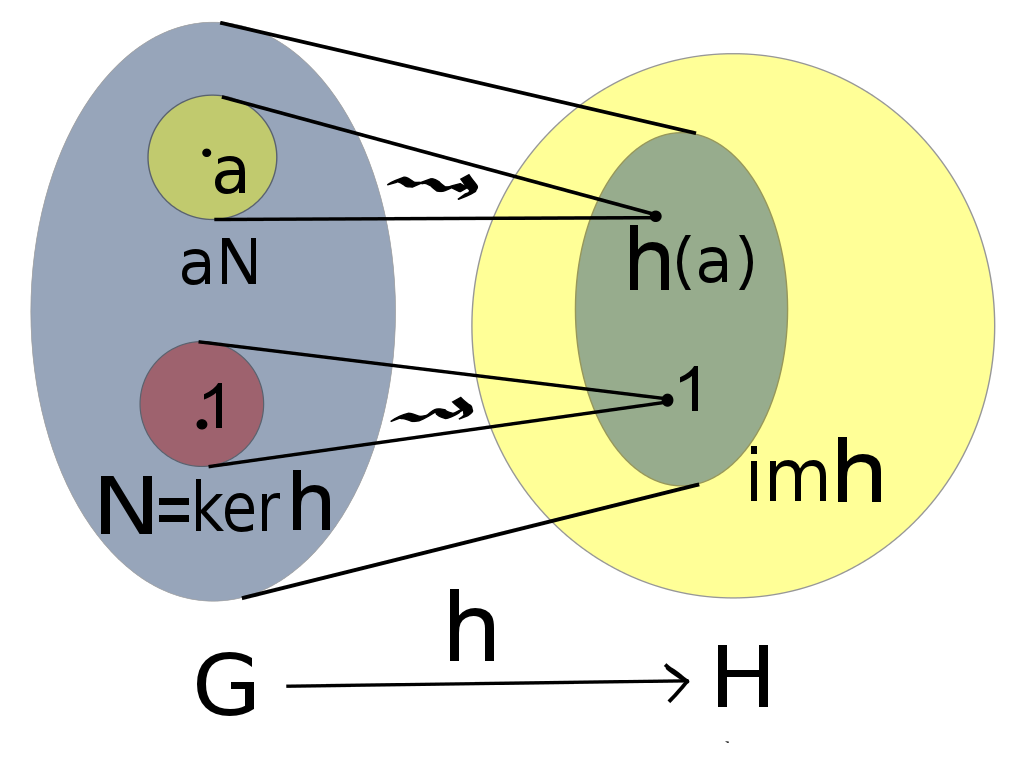
\includegraphics[width=0.8\textwidth]{img/group_homomorphism}
  \caption[labelInTOC]{
  Animation af en gruppehomomorfi $h: G \rightarrow H$. Den lille oval inde i
  $H$ er billedet af $H$. $N$ er kernen af $H$ og $aN$ er en sideklasse til
  $N$.}
  \label{figureLabel}
\end{center}
\end{figure}

\subsubsection{Prop. 2.4.9}
\label{2.4.9}
Lad $f: G \rightarrow K$ være en gruppehomomorfi. Så gælder:
\begin{enumerate}[(i)]
  \item Billedet $f(G) \subseteq K$ er en undergruppe til $K$.
  \item Kernen $Ker(f) \subseteq G$ er en normal undergruppe (\nameref{2.3.2}) til
  $G$.
  \item $f$ er injektiv (one-to-one) $\iff$ $Ker(f) = \{e\}$.
\end{enumerate}

\subsubsection{Gruppeisomorfi}
\label{gruppeisomorfi}
\begin{enumerate}[(i)]
    \item En bijektiv gruppehomomorfi kaldes en gruppeisomorfi.
    \item Vi bruger notationen $f: G \tilde{\rightarrow} K$.
    \item Vi skriver $G \tilde{=} K$ og siger $G$ og $K$ er isomorfe.
\end{enumerate}

\subsection{Isomorfisætningen  (2.5.1)}
\label{isomorfitheorem}
Lad $G$ og $K$ være grupper og $f: G \rightarrow K$ en gruppehomomorfi med
kernen $N = Ker(f)$. Så er:
\begin{equation*}
  \tilde{f}: G/N \rightarrow f(G)
\end{equation*}
givet ved $\tilde{f}(gN) = f(g)$ en afbildning og en gruppeisomorfi.

\textit{Da N er normal er $G/N$ en kvotientgruppe. Denne indeholder alle
sideklasser for N. $\tilde{f}$ afbilder fra disse sideklasser til billedet af
$f$ (dvs. alle elementer i $K$ der bliver afbildet af $f$). Man finder oftest
først en onto gruppehomomorfi $f: G \rightarrow K$ for en passende gruppe $K$,
sådan at $N = ker(f)$, så giver sætningen gruppeisomorfien $\tilde{f}$.}

\subsection{Orden af et element i en gruppe (2.6)}
\subsubsection{Prop. 2.6.1}
\label{2.6.1}
Lad $G$ være en gruppe og $g \in G$. Afbildningen
\begin{equation*}
  f_g: \Z \rightarrow G
\end{equation*}
givet ved $f_g(n) = g^n$ er en gruppehomomorfi fra $(\Z, +)$ til $G$.

\textit{Denne afbildning er den kendte potensopløftning (med + som komposition),
og det er en gruppehomomorfi (\nameref{2.4.1}.})

\subsubsection{Ordnen af et element}
\label{ord(g)}
\begin{enumerate}[(i)]
  \item Billedet $f_g(\Z) = \{g^n | n \in \Z\}$ skrives $\langle g \rangle$.
  \item $\langle g \rangle$ er en abelsk undergruppe af $G$.
  \item Antallet af elementer i $\langle g \rangle$ kaldes ordnen af $g$ og
  skrives $ord(g)$.
  \item $ord(g)$ kan man tænke på som den mindste positive potens af $g$ der
  giver $e$.
  \item Hvis sådan en potens ikke findes siges $g$ at have uendelig orden.
\end{enumerate}

\subsubsection{Prop. 2.6.3}
Lad $G$ være en endelig gruppe og lad $g \in G$. Så gælder:
\begin{enumerate}[(i)]
  \item $ord(g)$ dividerer $|G|$
  \item $g^{|G|} = e$
  \item Hvis $g^n = e$ for et $n > 0$ så $ord(g)|n$.
\end{enumerate}

\subsubsection{Supplement til 2.6}
Lad $G$ være en gruppe og $g \in G$. Betragt afbildningen $f_g: \Z \rightarrow
G$ (\nameref{2.6.1}). Der findes nu et heltal $n_g > 0$ sådan at $Ker(f_g) = n_g\Z$
(\nameref{2.2.3}). Fra dette kan vi konkludere
\begin{enumerate}[(i)]
  \item Hvis $n_g = 0$ er $f_g$ injektiv (one-to-one).
  \item Hvis $n_g > 0$, så er $g_n = g_m \iff n \mycong{m}{n_g}$. Dette medfører
  at
  \\
  $\langle g \rangle = \myset{g^0 = e, g^1 = g, g^2, \ldots, g^{n_g -1} }$
\end{enumerate}

Der gælder desuden at
\begin{equation*}
  f(g_n) = f(g)^n \quad \text{for alle g $\in G$ og alle $n \in \Z$}
\end{equation*}

\textit{Hvis $Ker_(f_g) = {0}$ er dette det kun $0 \in \Z$ der afbilder til $e
\in G$ og derved afbilder de andre elementer i $\Z$ til forskellige elementer i
$G$. Hvis $n_g > 0$ så afbilder kongruente heltal $\in \Z$ til det same element
i $G$. Derved giver det kun mening at potensopløfte elementer i $g$ med tal fra
$[0;n_g[$, da billedet af $f_g$ kun består af multiplum as disse.}

\subsection{Cykliske grupper (2.7)}
\subsubsection{Def. 2.7.1}
En cyklisk gruppe er en gruppe $G$, indeholdende et element $g$, sådan at $G =
\langle g \rangle$. Elementet $g$ kaldes en frembringer for $G$ og vi siger $g$
genererer $G$.

\textit{Hvis alle elementer i $G$ kan skrives som potenser af $g$ er $G$
cyklisk.}

\subsubsection{Prop 2.7.2}
En gruppe $G$ med primtalsorden $|G| = p$ er isomorf (\nameref{gruppeisomorfi}) til
den cykliske gruppe $\Z/p\Z$ (\nameref{kvotientgruppe}).

\textit{Dvs. hvis $G$ har en primtalsordenen $p$, så eksisterer der en isomorfi
$f: \Z/p\Z \rightarrow G$. Dette kommer af \nameref{isomorfitheorem}}

\subsubsection{Prop 2.7.4}
Lad $G$ være en cyklisk gruppe. Så gælder:
\begin{enumerate}[(i)]
  \item Enhver undergruppe af $G$ er cyklisk.
  \item Antag $G$ er endelig og at $d$ er en divisor i $|G|$. Så indeholder $G$
  en entydig undergruppe $H$, hvor $|H| = d$.
  \item Der er $\phi(d)$ elementer af orden $d$ i $G$. Disse er generatorerne
  for $H$.
\end{enumerate}
\textit{Eksempel: Lad $G = \Z/6\Z =
\myset{[0]_6,[1]_6,[2]_6,[3]_6,[4]_6,[5]_6}$. Det ses at $ord(G) = 6$, vi lader
derfor $d = 3$. En undergruppe skal indeholde det neutrale element $[0]_6$, så
denne skal være indeholdt.}

\textit{Dernæst skal hvert element i en undergruppe have en invers. Vi ved også at
enhver undergruppe af $G$ er cyklisk, de to elementer der tilfredsstiller
disse krav er $[2]_6$ og $[4]_6$. Dvs. $H = \myset{[0]_6,[2]_6,[4]_6}$.}

\textit{(iii) siger nu at der skal være 2 elementer i $G$ af ordnen 3. Det første
element der tilfredsstiller dette er $[2]_6$, da $[2]_{6}^3 = [0]_6$. Det andet
element er $[4]_6$, da $[4]_{6}^3 = [0]_6$. Ingen af de andre elementer har
denne egenskab.
(iii) siger nu at $[2]_6$ og $[4]_6$ genererer netop $H$.}

\subsubsection{Kor. 2.7.6}
Lad $N > 0 \in \Z$. Så gælder:
\begin{equation*}
  \sum_{d|N} \phi(d) = N
\end{equation*}
hvor der summeres over $d \in div(N)$.

\textit{Eksempel: Lad $N = 6$. $div(N) = div(6) = \myset{1,2,3,6}$. Nu siger
korollaret at $N = \phi(1) + \phi(2) + \phi(3) + \phi(6) = 1 + 1 + 2 + 2 = 6$.}

\subsection{Grupper og tal (2.8)}
\subsubsection{Produktgrupper}
Hvis $G_1, G_2,\ldots,G_n$ er grupper, så har produktet:
\begin{equation*}
  G = G_1 \times G_2 \times \cdots \times G_n = \{(g_1,g_2,\ldots,g_n) | g_1 \in
  G_1, g_2 \in G_2,\ldots g_n \in G_n \}
\end{equation*}
den naturlige komposition

\begin{equation*}
  (g_1, g_2,\ldots,g_n)(h_1,h_2,\ldots,h_n) = (g_1 h_1,g_2 h_2, \ldots, g_n h_n)
\end{equation*}
\textit{En produktgruppe skal ses som en gruppe indeholdende tupler, bestående
af et element fra hver faktorgruppe. To produktgrupper $G$ og $H$ komponeres
som vist ovenover.}

\subsubsection{Lemma 2.8.1}
Lad $M, N$ være normale undergrupper (\nameref{2.3.2}) af en gruppe $G$, hvor $M
\cap N = \{e\}$. Så er:
\begin{enumerate}[(i)]
  \item $MN$ en undergruppe til $G$.
  \item $\pi: M \times N \rightarrow MN$, givet ved $\pi(x,y) = xy$, en
  isomorfi.
\end{enumerate}

\subsubsection{Sprunget gruppeversioner af Euler og kineseren over}


\subsection{Symmetriske gruppe (2.9)}
\textit{Den symmetriske gruppe $S_n$ har som elementer alle permutationer af
bijektioner der afbilder fra tupler bestående af $n$ symboler til sig selv.
Altså en gruppe bestående af alle kombinationer af bijektioner over de $n$
symboler. Elementerne i $S_n$ kaldes permutationer. Gruppen \nameref{S_3} er et
eksempel på en symmetrisk gruppe.}

Der gælder at $|S_n| = n!$

\subsubsection{Def. 2.9.1}
Antag $\sigma \in S_n$. Så definerer vi
\begin{equation*}
  M_\sigma = \{x \in M_n | \sigma(x) \neq x\}
\end{equation*}
hvor $M_n = \{ 1, 2, \ldots, n \}$. Permutationerne $\sigma, \tau \in S_n$
kaldes disjunkte hvis $M_\sigma \cap M_\tau = \emptyset$.

\textit{$\sigma$ og $\tau$ er elementer i $S_n$, altså bijektioner over $M_n$.
$M_\sigma$ og $M_\tau$ er mængderne bestående af de tal som henholdsvist
$\sigma$ og $\tau$ permuterer. $M_\sigma \cap M_\tau = \emptyset$ hvis $\sigma$
og $\tau$ permuterer forskellige tal}.

\subsubsection{Prop 2.9.2}
Lad $\sigma, \tau \in S_n$ være disjunkte permutationer. Så gælder:
\begin{equation*}
  \sigma \tau = \tau \sigma
\end{equation*}
samt at $M_{\sigma\tau} = M_\sigma \cup M_\tau$

\subsubsection{$k$-cykel}
\label{$k$-cykel}
Antag vi er givet $k$ forskellige elementer i $M_n$. En permutation $\sigma \in
S_n$, givet ved:
\begin{equation*}
  \sigma(x_1) = x_2, \quad \sigma(x_2) = x_3, \quad \ldots, \quad \sigma_{k-1} =
  x_k, \quad \sigma(x_k) = x_1
\end{equation*}
og $\sigma(x) = x$ hvis $x \nin \{x_1,\ldots,x_k\}$ kaldes en $k$-cykel. Sådan
en cykel skrives $\sigma(x_1 x_2 \ldots x_k)$.

Bemærk at $M_\sigma = \{x_1, x_2, \ldots, x_k \}$ og at ordnen af en $k$-cykel i
$S_n$ er $k$. Se \nameref{ord(g)}.

\textit{Altså er en $k$-cykel en permutation der gør at alle $k$ elementer bliver
flyttet en frem og hvor det sidste element bliver flyttet til starten. De
andre ikke-k elementer i $M_n$ permuterer en $k$-cykel ikke. Tænk linked
list.}
 
\subsubsection{Prop 2.9.5}
Lad $\sigma \in S_n$ være skrevet som et produkt af disjunkte cykler $\sigma_1
\cdots \sigma_r$. Så er $ord(\sigma) = lcm(ord(\sigma_1), \cdots,
ord(\sigma_r))$. Se \nameref{ord(g)}.

\subsubsection{Prop 2.9.6}
Alle permutationer $\sigma \in S_n$ er et produkt af entydige disjunkte cykler.

\subsubsection{Lemma 2.9.8}
Antag $(i_1 i_2 \ldots i_k)$ er en $k$-cykel (\nameref{$k$-cykel}) og at $\sigma \in
S_n$ er en vilkårlig permutation. Så gælder:
\begin{equation*}
  \sigma(i_1 i_2 \ldots i_k)\sigma^{-1} =
  (\sigma(i_1)\sigma(i_2) \ldots \sigma(i_k))
\end{equation*}
\textit{Lemmaet fortæller, hvordan man beregner en konjugering af en $k$-cykel.
Eksempel: Hvis vi vil konjugere 3-cyklen $(1 2 3)$ med permutationen $\sigma =
(1 2 5)(3 4)$ i $S_5$, dvs hvis vi vil udregne $\sigma$ (1 2 3) $\sigma^{-1}$,
så behøver vi blot at finde $\sigma(1)=2$, $\sigma(2)=5$ og $\sigma(3)=4$.
Lemmaet siger nu at $\sigma (1 2 3) \sigma^{-1} = (\sigma(1) \sigma(2)
\sigma(3)) = (2 5 4)$. Vi slipper altså for at beregne $\sigma^{-1}$.}

\subsubsection{Simple transpositioner}
\label{simple_trans}
En 2-cykel kaldes en transposition i $S_n$. Pga det er en 2-cykel er en
transposition sin egen invers. En simpel transposition er en transposition på
følgende form:
\begin{equation*}
  s_i = (i \quad i + 1)
\end{equation*}
hvor $i = 1,\ldots, n-1$

\textit{Altså er en simpel transposition en transposition der permuterer et
symbol $i$, en plads frem. $i$ kan ligge i intervallet $1 \leq i < n $.}

\subsubsection{Bubble sort}
Simpel sorteringsalgoritme. Går igennem elementerne en ad gangen og sammenligner
naboparrene, hvis et efterfølgende element er skarpt større end det forrige
swappes disse og algoritmen starter forfra. Når algoritmen når til sidste
element er elementerne sorterede. Disse swaps er eksempler på simple
transpositioner.

\subsubsection{Def. 2.9.10}
\label{2.9.10}
Lad $\sigma \in S_n$ være en permutation. Et par af indekser $(i, j)$, hvor $1
\leq i < j \leq n$, kaldes en \textbf{inversion} af $\sigma$, hvis $\sigma(i) >
\sigma(j)$.

\textit{Et par (i, j), hvor i er mindre end j, men hvor permutationen $\sigma$
gør at $\sigma(i) > \sigma(j)$ kaldes en inversion af $\sigma$.}

Lad
\begin{equation*}
  I_\sigma = \myset{(i,j) | 1\leq i < j \leq n \myand \sigma(i) > \sigma(j)}
\end{equation*}
være mængden af alle inversioner og lad $n(\sigma) = |I_\sigma|$ være antallet
af inversioner af $\sigma$.

\subsubsection{Prop 2.9.12}
Permutationen $\sigma \in S_n$ er identitetsafbildningen $\iff n(\sigma) = 0$.
Hvis $\sigma$ ikke er identitetsafbildningen så eksisterer der et $1 \leq i < n$
sådan at $\sigma(i) > \sigma(i + 1)$.

\textit{Identitetsafbildningen er den eneste permutation der ingen inversioner
har. Hvis $\sigma$ ikke er identitetsafbildningen så eksisterer der en
inversion af $\sigma$ for et nabopar $(i, j)$, altså hvor $j = i + 1$.}

\subsubsection{Lemma 2.9.13}
Lad $s_i \in S_n$ være en simpel transposition (\nameref{simple_trans}) og $\sigma
\in S_n$. Så gælder:
\begin{equation*}
n(\sigma s_i) = \left\{
\begin{array}{l l}
n(\sigma) + 1 & \quad \text{hvis $\sigma(i) < \sigma(i + 1)$}\\
n(\sigma) - 1 & \quad \text{hvis $\sigma(i) > \sigma(i + 1)$}\\
\end{array} \right.
\end{equation*}

\textit{Lemmaet siger at antallet af inversioner af $\sigma$ komponeret med den
simple transposition $s_i$, er lig $n(\sigma) \pm 1$ afhængigt af om $(i, i +
1)$ er en inversion af $\sigma$ eller ej.}

\subsubsection{Lemma 2.9.14}
Lad $\sigma \in S_n$. Så gælder:
\begin{enumerate}[(i)]
  \item $\sigma$ er et produkt af $n(\sigma)$ simple transpositioner.
  \item $n(\sigma)$ er det mindste antal simple transpositioner der skal bruges
  for at skrive $\sigma$ som et produkt af simple transpositioner.
\end{enumerate}

\subsubsection{Def. 2.9.15}
Fortegnet af en permutation $\sigma \in S_n$ er
\begin{equation*}
  sgn(\sigma) = (-1)^{n(\sigma)}
\end{equation*}
En permutation med positivt fortegn kaldes lige, en permutation med negativt
fortegn kaldes ulige.

\textit{Antallet af inversioner (\nameref{2.9.10}) af en permutation afgør om den er
lige eller ulige.}

\subsubsection{Prop 2.9.16}
\label{2.9.16}
Afbildningen
\begin{equation*}
  sgn: S_n \rightarrow \myset{\pm 1}
\end{equation*}
er en gruppehomomorfi, hvor kompositionen i $\myset{\pm 1}$ er multiplikation.

\subsubsection{Den alternerende gruppe}
Mængden af lige permutationer i $S_n$ skrives $A_n$ og kaldes den alternerende
gruppe. Fra \nameref{2.9.16} og \nameref{2.4.9} (ii) kan vi konkludere at $A_n$ er en
normal undergruppe til $S_n$, da $A_n$ netop er kernen til afbildningen $sgn$.
Der gælder at $|A_n| = n! / 2$.

\subsubsection{Prop 2.9.17}
Lad $n \geq 2$. En transposition (\nameref{simple_trans}) $\tau = (i \quad j) \in
S_n$ er en ulige permutation. Fortegnet af en r-cykel $\sigma = (x_1 x_2 \ldots
x_r)$ er $(-1)^{r-1}$.

\subsubsection{Simple grupper}
\label{simple-grupper}
En gruppe $N$ kaldes simpel hvis $\myset{e}$ og $N$ er de eneste normale
undergrupper (\nameref{2.3.2}) af $N$.

\subsubsection{Lemma 2.9.18}
Enhver permutation i $A_n$ er et produkt af en 3-cykel hvis $n \geq 3$.

\subsubsection{Sætning 2.9.19}
Den alternerende gruppe $A_n$ er simpel for $n \geq 5$.

\subsubsection{Lemma 2.9.20}
Enhver 3-cykel er et produkt af en simpel 3-cykler i $A_n$ hvis $n \geq 3$.

En 3-cykel kaldes simpel hvis den er på formen $(k \quad k + 1 \quad k + 2)$.

\subsection{Gruppevirkninger (2.10)}
\subsubsection{Def. 2.10.1}
\label{2.10.1}
Lad $G$ være en gruppe og $S$ en mængde. Vi siger at $G$ virker på en gruppe
hvis der eksisterer en afblidning
\begin{equation*}
  \alpha: G \times S \rightarrow S
\end{equation*}
som skrives $\alpha(g,s) = g \cdot s$ sådan at:
\begin{enumerate}[(i)]
  \item $e \cdot s = s$ for alle $s \in S$
  \item $(g \cdot h) s = g (h \cdot s)$ for alle $g,h \in G$ og for alle $s \in
  S$.
\end{enumerate}

\textit{En virkning er en afbildning der afbilder fra et element $s \in S$ og et
gruppeelement $g \in G$, til $S$. Denne afbildning skal respektere det neutrale
element og være associativ.}

\subsubsection{Def. 2.10.2}
\label{2.10.2}
Lad $\alpha: G \times S \rightarrow S$ være en virkning af $G$ på $S$ og $s \in
S$ et element i $S$. Så er:
\begin{equation*}
  G \cdot s = Gs = \myset{gs|g \in G}
\end{equation*}
\textbf{banen} af $s$ under virkningen af $G$. Mængden af baner
$\myset{Gs|s \in S}$ skriver vi $S/G$.

\textit{Banen af $s$ under $G$  $\subseteq S$ er den delmængde af $S$ som
$\alpha$ afbilder dette $s$ og hele $G$ til.}

Lad $X \subseteq S$ være en delmængde af $S$ og $g \cdot X = gX = \myset{gx|x
\in X}$, hvor $g \in G$. Så er:
\begin{equation*}
  G_X = \myset{g \in G|gX = X}
\end{equation*}
\textbf{stabilisatoren} for $X$. Hvis $X = \myset{x}$ skrives $G_X$ som
$G_x$.

\textit{Stabilisatoren $G_X \subseteq G$ er den delmængde hvis virkning
ikke ændrer elementerne i $X$}.

Et \textbf{fikspunkt} for en virkning er et element $s \in S$ sådan at $gs = s$
for alle $g \in G$. Mængden af fikspunkter skriver vi $S^G$.

\textit{Et fikspunkt er et element $s \in S$ der er neutral mht. $G$s virkning.}

\subsubsection{Prop. 2.10.5}
Lad $\alpha: G \times S \rightarrow S$ være en virkning. Så gælder:
\begin{enumerate}[(i)]
  \item Lad $X \subseteq S$ være en delmængde af $S$. Så er $G_X$ en undergruppe
  af $G$.
  \item Mængden $S$ er foreningen af $G$-baner:
  \begin{equation*}
  S = \bigcup_{s \in S}Gs
  \end{equation*}
  hvor $Gs \neq Gt \Rightarrow Gs \cap Gt = \emptyset$ hvis $s, t \in S$.
  \item Lad $x \in S$. Så er
  \begin{equation*}
  \tilde{f}: G/G_x \rightarrow Gx
  \end{equation*}
  givet ved $\tilde{f}(gG_x) = gx$ en veldefineret bijektiv afbildning fra
  $G_x$'s venstre sideklasser til banen $Gx$.
\end{enumerate}

\subsubsection{Kor. 2.10.7}
\label{2.10.7}
Lad $G \times S \rightarrow S$ være en virkning hvor $S$ er endelig. Så gælder:
\begin{equation*}
  |S| = |S^G| + \sum_x |G/G_x|
\end{equation*}
hvor der summes ved at vælge et element $x$ fra hver bane med mere end et
element.

\textit{Ordnen af $S$ er lig antallet af fikspunkter + summen af antallet af
venstre sideklasser (\nameref{sideklasser}) for hvert element i $G_x$, altså de
elementer der er stabile under konjugering med $x$.}

\subsubsection{Lemma 2.10.8 (Burnside)}
Lad $G \times S \rightarrow S$ være en virkning, hvor $G$ er en endelig gruppe
og $S$ en endelig mængde. Så gælder:
\begin{equation*}
  |S/G| = \frac{\sum_{g \in G}|S^g|}{|G|}
\end{equation*}
hvor $S^g = \myset{x \in S| gx = x}$.

\textit{$S^g$ er de elementer i $S$ der er fikspunkter under $g$. Antallet af
baner for en virkning er altså lig summen af antallet af fikspunker under $g$
divideret med ordnen af $G$. Sagt med andre ord, antallet af baner (et
naturligt tal eller $+\infty$) er lig det gennemsnitlige antal fikspunkt under
et element af $g$.}

\subsubsection{Konjugering}
\label{konj}
Afbildningen $\alpha: G \times G \rightarrow G$ givet ved $\alpha(g,h) =
ghg^{-1}$ er en virkning af G på G. Den kaldes konjugering.

$C(h)$ kaldes konjugeringsklassen indeholdende $h$ og udgør banen (\nameref{2.10.2}) 
\begin{equation*}
  C(h) = G \cdot h = \myset{ghg^{-1}|g\in G}
\end{equation*}

\textit{Altså er konjugeringsklassen indeholdende $h$ en delmængde af $G$
indeholdende de elementer som $ghg^{-1}$ afbilder til. I en abelsk gruppe er
enhver konjugeringsklasse en singleton}.

$Z(h)$ kaldes centralisatoren af $h$ og udgør stabilisatoren (\nameref{2.10.2})
$G_h$:
\begin{equation*}
  Z(h) = \myset{g \in G | gh = hg}
\end{equation*}

\textit{Altså er centralisatoren af $h$ mængden af elementer i $G$ hvor
$ghg^{-1} = hgh^{-1}$.}

$Z(G)$ kaldes centeret af $G$ og udgør mængden af fikspunkter for $G$:
\begin{equation*}
  Z(G) = G^G = \myset{g \in G|gx = xg \text{ for alle }x \in G}
\end{equation*}

\textit{$Z(G)$ er altså mængden af elementer der er stabile med alle elementer i
$G$ under konjugering. $Z(G)$ er en normal abelsk undergruppe af $G$ og
indeholder mindst elementet $e$ for konjugeringsvirkningen.}

Hvis $G$ er en endelig gruppe kan vi skrive \nameref{2.10.7} som:
\begin{equation*}
  |G| = |Z(G)| + \sum_{h \in G}|G/Z(h)|
\end{equation*}

\textit{Ordnen af $G$ er lig antallet af fikspunkter for $G$ + summen af
antallet af venstre sideklasser (\nameref{sideklasser}) for elementerne i $G_h$,
altså de elementer der er stabile under konjugering med $h$.}

$N_G(H)$ kaldes normalisatoren af $H$ i $G$ og udgør stabilisatoren af
undergruppen $H \subseteq G$:
\begin{equation*}
  N_G(H) = G_H = \myset{g \in G | gHg^{-1} = H}
\end{equation*}

\textit{$H$ er normal $\iff N_G(H) = G$}.

\subsubsection{$p$-gruppe}
\label{p-gruppe}
En endelig gruppe med orden $p^r$, hvor $p$ er et primtal og $r \in \N$ kaldes
en $p$-gruppe.

\subsubsection{Prop. 2.10.13}
Lad $G$ være en ikke-triviel $p$-gruppe virkende (\nameref{2.10.1}) på en mængde $S$.
Så er 
\begin{equation*}
  |S| \mycong{|S^G|}{p}
\end{equation*}

\textit{Ordnen af $S$ er kongruent $(mod$  $p)$ til antallet af fikspunkter i
$S$ under $G$, hvis $G$ er en ikke-triviel $p$-gruppe.}

\subsubsection{Kor. 2.10.14}
Lad $G$ være en ikke-triviel $p$-gruppe med orden $p^r$, så er
\begin{equation*}
  |G| \mycong{|Z(G)|}{p}
\end{equation*}
og $|Z(G)| > 1$.

\textit{Ordnen af $G$ er kongruent $(mod$  $p)$ til størrelsen af centeret af
$G$ (\nameref{konj}), altså antallet af fikspunkter for $G$, samt centeret af
$G$ består af mere end 1 element.}

\subsubsection{Kor. 2.10.15}
Lad $p$ være et primtal. En gruppe $G$ med orden $|G| = p^2$ er abelsk.

\subsubsection{Def. 2.10.16 (Sylow $p$-undergruppe)}
\label{sylow-$p$-undergruppe}
Lad $G$ være en endelig gruppe og $p$ et primtal. Antag nu at $|G| = p^r m$,
hvor $p \not | m$. En undergruppe $H \subseteq G$ med orden $|H| = p^r$ kaldes
en Sylow $p$-undergruppe.

\textit{Hvis en $p$-gruppe (\nameref{p-gruppe}) $H \subseteq G$ og $|G| = p^r m$,
hvor $p \not | m$, kaldes $H$ en Sylow $p$-undergruppe.}

\subsubsection{Sætning 2.10.17 (Første Sylow Sætning)}
Lad $G$ være en endlig gruppe og $p$ et primtal. Antag at $|G| = p^r m$, hvor $p
\not | m$. Så indeholder $G$ en Sylow $p$-undergruppe.

\subsubsection{Sætning 2.10.18 (Anden Sylow Sætning)}
Lad $G$ være en endelig gruppe og $P, Q$ to Sylow $p$-undergrupper. Så
eksisterer der et $g \in G$ sådan at:
\begin{equation*}
  gPg^{-1} = Q
\end{equation*}
Ydermere, enhver $p$-undergruppe $H$ (\nameref{p-gruppe}) er indeholdt i en Sylow
$p$-undergruppe.

\textit{Hvis $P, Q$ er to Sylow $p$-undergruppe, har de samme orden. Da der
eksisterer et $g \in G$ sådan at $gPg^{-1} = Q$ siger vi at $P$ og $Q$ tilhører
samme konjugeringsklasse (\nameref{konj}.})

\subsubsection{Sætning 2.10.19 (Tredje Sylow Sætning)}
Lad $G$ være en endelig gruppe med orden $p^r m$, hvor $p \nmid m$. Lad $Syl_p
(G)$ være mængden af Sylow $p$-undergrupper. Så gælder:
\begin{enumerate}[(i)]
  \item $|Syl_p (G)|$ dividerer m.
  \item $|Syl_p (G)| \mycong{1}{p}$
\end{enumerate}
Eksempler på brugen af Sylow sætningerne kan ses på side 103.

\subsubsection{Supplement til 2.10. Lemma}
Lad $G$ være en gruppe og $g \in G$. Afbildningen 
\begin{equation*}
  i_g: G \rightarrow G
\end{equation*}
givet ved $i_g (x) = gxg^{-1}$ kaldes konjugering med $g$.

Afbildningen $i_g$ er en gruppeisomorfi. Dette medfører:
\begin{enumerate}[(i)]
  \item Hvis $H$ er en undergruppe af $G$, så er $i_g (H)$ en undergruppe af
  $G$.
  \item $ord(x) = ord(gxg^{-1})$ for alle $x \in G$.
\end{enumerate}

\subsubsection{Supplement til 2.10. Korrolar}
Lad $p$ være et primtal og lad $G$ være en endelig $p$-gruppe (\nameref{p-gruppe})
med $|G|> p$. Så er $G$ ikke simpel \nameref{simple-grupper}.

\subsubsection{Supplement til 2.10. Observation}
Lad $G$ være en endelig gruppe og $p$ et primtal. Hvis $G$ kun har een Sylow
$p$-undergruppe $P$ (\nameref{sylow-$p$-undergruppe}), så er $P$ en normal undergruppe af $G$.

\subsubsection{Supplement til 2.10. Lemma}
Lad $G$ være en endelig gruppe og lad $p$ og $q$ være to entydige primtal. Lad
$P$ være en Sylow $p$-undergruppe af $G$ og $Q$ en Sylow $q$-undergruppe af $G$.
Så gælder:
\begin{enumerate}[(i)]
  \item $P \cap Q = \myset{e}$
  \item Hvis $P$ og $Q$ er normale i G (\nameref{2.3.2}), så er $xy = yx$ for alle
  $x \in P$ og $y \in Q$
  \item Hvis $p$ og $q$ er de eneste primdivisorer af $|G|$, og hvis enten $P$
  eller $Q$ er normale i $G$, så $G = PQ$.
\end{enumerate}

\newpage